% Provenance (never printed): see sources/outline_sources.md (Year 2: mid-latitude cyclones and
% fronts; jets and Rossby waves, descriptive; tropical cyclones; numerical weather prediction,
% principle). Definitions after the NWS glossary and UCAR; cyclogenesis conditions after the NOAA
% AOML FAQ; potential intensity after Gilford (2021, pyPI); conveyor belts after Raveh-Rubin and
% Catto (2019); blocking after Wang and others (2026); predictability after Krishnamurthy (2019),
% Selz and others (2022) and ECMWF. The Lorenz system from figdata/bachelor-2/weather.py; the
% fronts, waves and storms of the examples, exercises and problem are invented, their values
% computed in the Book 4 scratch calculator calc/ch22.py.
\chapter{Systèmes météorologiques}\label{ch:b2:weather-systems}

Une prévision à quatre jours est aujourd'hui aussi fiable qu'une prévision à un jour l'était il y a trente
ans, et chaque décennie a ajouté environ un jour de prévision utile. Pourtant, aucune prévision du temps
d'un jour donné, en un lieu donné, n'est fiable bien au-delà de dix jours, et de meilleurs ordinateurs
ne suffiront pas à repousser beaucoup cette limite~: l'atmosphère amplifie ses propres petites incertitudes. Ce
chapitre décrit les systèmes météorologiques que suivent les prévisions, les fronts et les dépressions
des moyennes latitudes, les ondes du courant-jet et les cyclones tropicaux, puis la manière dont ils sont
prévus et pourquoi la prévision doit s'arrêter quelque part.
% ledger: mo:accuracy, bauer:day-per-decade, krish19:predictability

\begin{recall}
\textbf{Des volumes scolaires}~: masses d'air, fronts, fronts froids et chauds, dépressions et
anticyclones, isobares et prévisions du temps ; le cyclone tropical, son œil et son mur de l'œil, l'échelle de
Saffir--Simpson. \textbf{Du volume de première année}~: la force du gradient de pression, le paramètre de
Coriolis $f = 2\Omega\sin\varphi$, l'équilibre géostrophique, les cyclones et anticyclones, les trois
cellules, les vents d'ouest et les courants-jets. \textbf{Des volumes de physique}~: les moteurs thermiques
et le rendement d'un cycle de Carnot. \textbf{Du \cref{ch:b2:atmospheric-thermodynamics}}~:
saturation, \omterm{def:b2:atmospheric-thermodynamics:moist-adiabat}{adiabatique humide}, $\theta_e$, \omterm{def:b2:atmospheric-thermodynamics:instability}{instabilité conditionnelle} et CAPE.
\end{recall}

\section{Fronts}\label{sec:b2:weather-systems:fronts}

Les volumes scolaires dessinaient les fronts comme des lignes sur une carte. Un front est la ligne où une
surface inclinée qui sépare deux masses d'air rencontre le sol, et le temps qu'il apporte vient de cette pente.

\begin{definition}[Surface frontale~; front stationnaire~; front occlus]\label{def:b2:weather-systems:fronts}
La \emph{surface frontale}\index{surface frontale} d'un front est la limite inclinée entre les deux masses d'air,
la plus dense et la plus froide restant dessous en forme de coin ; le front sur la carte en est l'intersection avec le sol. Un
\emph{front stationnaire}\index{front stationnaire} est un front qui se déplace très lentement ou pas du tout. Un
\emph{front occlus}\index{front occlus} est un front composé de deux fronts, formé lorsqu'un front froid rattrape
un front chaud ou stationnaire.
\end{definition}
% ledger: nws4:front, nws4:stationary, nws4:occluded

Un \omterm{def:b2:weather-systems:fronts}{front stationnaire} se forme lorsqu'aucune des deux masses d'air ne peut pousser l'autre, les vents soufflant le long
du front plutôt qu'en travers ; il peut rester des jours, nuageux et pluvieux, avant de repartir en front froid
ou en front chaud. Sur une carte il alterne les triangles bleus d'un front froid, pointant vers l'air chaud, avec les
demi-cercles rouges d'un front chaud, pointant vers l'air froid. Un \omterm{def:b2:weather-systems:fronts}{front occlus} se dessine en violet avec les deux
symboles du même côté. Lorsque l'air situé derrière le front froid est le plus froid, il glisse sous le front
chaud et le soulève en altitude : c'est une occlusion froide ; lorsque l'air situé devant le front chaud est le plus
froid, le front froid remonte par-dessus lui : c'est une occlusion chaude.
% ledger: ucar4:stationary-occluded, nws4:occluded

Quelle est la pente d'une \omterm{def:b2:weather-systems:fronts}{surface frontale}~? La réponse relie l'équilibre hydrostatique à l'équilibre géostrophique
du volume de première année.

\begin{proposition}[Pente d'une surface frontale]\label{prop:b2:weather-systems:slope}
Soit une \omterm{def:b2:weather-systems:fronts}{surface frontale} séparant de l'air froid à la température $T_c$ de l'air chaud à $T_w$, avec des vents
géostrophiques $v_c$ et $v_w$ le long du front. Prenons l'axe $x$ en travers du front, vers l'air froid, et l'axe $y$
le long de celui-ci, de sorte que $(x, y, z)$ soit direct. Alors la \omterm{def:b2:weather-systems:fronts}{surface frontale} monte vers l'air froid
selon la pente
\[
  \tan\alpha \approx \frac{f\,\bar T\,(v_c - v_w)}{g\,(T_w - T_c)},
\]
où $\bar T$ est la température moyenne. Une \omterm{def:b2:weather-systems:fronts}{surface frontale} en équilibre exige un saut du vent le long d'elle,
$v_c > v_w$~: le vent tourne cycloniquement en travers du front.
\end{proposition}

\begin{proof}
La pression est continue à travers la \omterm{def:b2:weather-systems:fronts}{surface frontale}, donc sa variation le long de la surface est la
même des deux côtés~: $\partial_x p_c\,\mathrm{d}x + \partial_z p_c\,\mathrm{d}z =
\partial_x p_w\,\mathrm{d}x + \partial_z p_w\,\mathrm{d}z$. De chaque côté $\partial_z p = -\rho g$
(équilibre hydrostatique) et $\partial_x p = \rho f v$ (équilibre géostrophique). D'où
$\rho_c f v_c\,\mathrm{d}x - \rho_c g\,\mathrm{d}z = \rho_w f v_w\,\mathrm{d}x - \rho_w
g\,\mathrm{d}z$, et
\[
  \frac{\mathrm{d}z}{\mathrm{d}x} = \frac{f(\rho_c v_c - \rho_w v_w)}{g(\rho_c - \rho_w)} .
\]
À même pression, $\rho \propto 1/T$, donc $\rho_c - \rho_w \approx \bar\rho\,(T_w -
T_c)/\bar T$~; au numérateur, la petite différence des masses volumiques peut être négligée, ce qui
donne la formule. L'air froid se trouve dessous, donc la surface monte vers lui, $\mathrm{d}z/
\mathrm{d}x > 0$, et $v_c > v_w$. Avec $x$ dirigé vers l'air froid, la vorticité relative
$\partial v/\partial x$ en travers du front est alors positive~: cyclonique.
\end{proof}

\begin{example}[Une pente typique]\label{ex:b2:weather-systems:slope}
À \ang{45}~N, $f = \qty{1.03e-4}{s^{-1}}$. À travers un front où $\bar T = \qty{280}{K}$, avec un écart
de température de \qty{5}{K} et un vent qui change de \qty{10}{m/s} le long du front, $\tan\alpha
= 1.03 \times 10^{-4} \times 280 \times 10/(9.81 \times 5) = 0.0059$, soit environ 1 sur 170~: la
\omterm{def:b2:weather-systems:fronts}{surface frontale} atteint une hauteur de \qty{1}{km} à environ \qty{170}{km} du front, au sol.
Un changement de vent plus brusque donne une surface plus raide ; un contraste de température plus fort, une surface plus douce.
\end{example}

Les fronts réels ont des pentes de cet ordre, et ce coin peu incliné explique leur temps. Devant un front
chaud, l'air chaud glisse sur une pente douce pendant des centaines de kilomètres~: d'abord arrivent les nuages
élevés, cirrus et cirrostratus, puis les altostratus, et les nuages s'épaississent et s'abaissent jusqu'à ce que la pluie
tombe près du front. Un front froid, plus raide et plus rapide, jusqu'à deux fois plus vite qu'un front
chaud, soulève brusquement l'air chaud : cumulus et cumulonimbus, averses, rafales et chute brutale
de température, la pression cessant de baisser et se mettant à monter au passage du front. Un front
où l'air chaud descend la \omterm{def:b2:weather-systems:fronts}{surface frontale} au lieu de la remonter s'appelle un katafront.
% ledger: ucar:warm-front, ucar:cold-front, nws4:front

\begin{omfigure}
\centering
\begin{tikzpicture}[font=\scriptsize, >=Stealth, x=1cm, y=1cm]
% air masses
\fill[omCold!12] (0,0) -- (0,3.4) .. controls (1.6,2.2) and (3.2,0.8) .. (4,0) -- cycle;
\fill[omCold!12] (9.6,0) .. controls (11,0.6) and (12.6,1.5) .. (14,2.4) -- (14,0) -- cycle;
\fill[omWarm!8] (4,0) .. controls (3.2,0.8) and (1.6,2.2) .. (0,3.4) -- (0,4.8) -- (14,4.8)
  -- (14,2.4) .. controls (12.6,1.5) and (11,0.6) .. (9.6,0) -- cycle;
% frontal surfaces
\draw[omCold, thick] (4,0) .. controls (3.2,0.8) and (1.6,2.2) .. (0,3.4);
\draw[omWarm, thick] (9.6,0) .. controls (11,0.6) and (12.6,1.5) .. (14,2.4);
% clouds
\fill[black!18, draw=black!45] (3.75,0.5) .. controls (3.5,1.8) and (3.7,3.2) .. (3.9,3.9)
  .. controls (3.2,4.15) and (3.0,4.5) .. (3.4,4.6) -- (5.8,4.6) .. controls (6.1,4.45) and
  (5.7,4.15) .. (5.1,3.9) .. controls (5.3,3.0) and (5.4,1.6) .. (5.05,0.5) -- cycle;
\node[align=center] at (4.45,2.6) {cumulo-\\nimbus};
\fill[black!15, draw=black!40] (9.6,0.35) .. controls (10.4,0.75) and (11.2,1.05) .. (11.9,1.25)
  -- (11.9,1.75) .. controls (11,1.6) and (10.2,1.35) .. (9.4,0.95) -- cycle;
\node at (10.75,1.25) [rotate=21] {nimbostratus};
\fill[black!10, draw=black!35] (11.9,1.35) .. controls (12.3,1.55) and (12.7,1.75) .. (13.0,1.9)
  -- (13.0,2.25) .. controls (12.6,2.1) and (12.2,1.95) .. (11.9,1.85) -- cycle;
\node[anchor=south] at (12.45,2.15) {altostratus};
\draw[black!40, line width=1.6pt] (12.9,2.75) -- (13.9,3.05);
\node[anchor=south] at (13.35,3.05) {cirrostratus};
\foreach \x in {12.2,12.7,13.2,13.7} {\draw[black!40, thick] (\x,3.95) .. controls (\x+0.15,4.05) .. (\x+0.35,3.9);}
\node[anchor=south] at (13.0,4.05) {cirrus};
% rain
\foreach \x in {3.95,4.25,4.55,4.85} {\draw[omCold!70, dashed] (\x,0.45) -- (\x-0.12,0.02);}
\foreach \x in {9.8,10.2,10.6,11.0,11.4} {\draw[omCold!70, dashed] (\x,0.55) -- (\x-0.12,0.02);}
% ground and labels
\draw[thick] (0,0) -- (14,0);
\node at (1.2,0.8) {air froid};
\node at (7.0,2.4) {secteur chaud};
\node at (12.8,0.55) {air froid};
\node[anchor=north, omCold] at (4,-0.05) {front froid};
\node[anchor=north, omWarm] at (9.6,-0.05) {front chaud};
\draw[->, thick] (6.0,0.55) -- (7.2,0.55) node[right] {les fronts se déplacent vers l'est};
\draw[->, black!60] (5.8,1.1) .. controls (7.0,1.4) and (9.5,2.0) .. (12.2,3.3);
\node[black!60, rotate=13] at (8.4,2.0) {l'air chaud glisse vers le haut};
\end{tikzpicture}
\par\smallskip{\small Coupe transversale à travers un front froid et un front chaud, ouest à gauche
(schéma~: l'échelle verticale est exagérée environ cent fois, et le front froid est dessiné plus raide que le front chaud).
Noms et succession des nuages comme dans le texte.}
\end{omfigure}
% ledger: ucar:warm-front, ucar:cold-front

\section{Cyclones extratropicaux}\label{sec:b2:weather-systems:cyclones}

\begin{definition}[Cyclone extratropical~; modèle du front polaire~; cyclogenèse]\label{def:b2:weather-systems:cyclones}
Un \emph{cyclone extratropical}\index{cyclone extratropical} est un cyclone des moyennes et hautes
latitudes, souvent large d'environ \qty{2000}{km}, qui porte en général des fronts, un front froid traînant
sur des centaines de kilomètres vers l'équateur. Le \emph{modèle du front polaire}\index{modèle du front polaire}
décrit sa vie comme une onde qui croît sur le front polaire, long front entre l'air polaire
et l'air tropical. La \emph{cyclogenèse}\index{cyclogenèse} est la formation ou le renforcement
d'un cyclone.
\end{definition}
% ledger: nws4:extratropical, nws4:polar-front

Le modèle suit un cyclone à travers quatre stades, comme le montre la figure ci-dessous. Un \omterm{def:b2:weather-systems:fronts}{front stationnaire}
sépare de l'air froid se déplaçant vers l'ouest, côté pôle, d'air chaud se déplaçant vers l'est, côté équateur.
Une perturbation courbe le front en onde ; la pression baisse à sa crête, une dépression se forme, et le front
à l'est de la dépression avance vers le pôle en front chaud, tandis que le front à l'ouest avance vers l'équateur
en front froid. Entre eux s'étend le secteur chaud. Le front froid va plus vite que le front chaud, et le secteur
chaud se rétrécit : le front froid rattrape le front chaud près de la dépression, et l'occlusion gagne depuis le centre
en soulevant l'air chaud hors du sol ; le cyclone, privé de son alimentation en air chaud, se comble et meurt.
Le point où les trois fronts se rejoignent s'appelle le point triple. Sur les images satellite, un cyclone mature
montre un nuage en forme de virgule
et une fente d'air sec et clair qui s'enroule sur son flanc sud et est.
% ledger: nws4:extratropical, nws4:occluded, ucar:cold-front

\begin{omfigure}
\centering
\begin{tikzpicture}[font=\scriptsize, >=Stealth]
% (a) stationary front
\begin{scope}[shift={(0,4.1)}]
\draw[black!30] (0,0) rectangle (6.4,3.4);
\node[anchor=north west] at (0,3.4) {\textbf{a}\enspace front stationnaire};
\draw[stationary front] (6.1,1.6) -- (0.3,1.6);
\draw[->, black!60] (4.2,2.5) -- (2.2,2.5); \node[black!60] at (3.2,2.8) {air froid};
\draw[->, black!60] (2.2,0.7) -- (4.2,0.7); \node[black!60] at (3.2,0.4) {air chaud};
\end{scope}
% (b) open wave
\begin{scope}[shift={(6.9,4.1)}]
\draw[black!30] (0,0) rectangle (6.4,3.4);
\node[anchor=north west] at (0,3.4) {\textbf{b}\enspace une onde et une dépression};
\fill[omWarm!10] (3.0,1.9) .. controls (3.9,1.75) and (4.8,1.55) .. (6.0,1.4) -- (6.0,0.2)
  -- (1.3,0.2) .. controls (2.0,0.9) and (2.6,1.4) .. (3.0,1.9) -- cycle;
\draw[black!45] (3.0,1.9) ellipse (0.55 and 0.4);
\draw[black!45] (3.0,1.9) ellipse (1.05 and 0.75);
\draw[warm front] (3.0,1.9) .. controls (3.9,1.75) and (4.8,1.55) .. (6.0,1.4);
\draw[cold front] (3.0,1.9) .. controls (2.6,1.4) and (2.0,0.9) .. (1.3,0.2);
\node[font=\small\bfseries, omWarm!70!black] at (2.7,2.15) {L};
\node at (4.5,0.75) {secteur chaud};
\end{scope}
% (c) mature
\begin{scope}[shift={(0,0)}]
\draw[black!30] (0,0) rectangle (6.4,3.4);
\node[anchor=north west] at (0,3.4) {\textbf{c}\enspace cyclone mature};
\fill[omWarm!10] (3.0,1.9) .. controls (3.9,1.7) and (4.8,1.5) .. (6.0,1.25) -- (6.0,0.2)
  -- (3.3,0.2) .. controls (3.3,0.8) and (3.2,1.45) .. (3.0,1.9) -- cycle;
\draw[black!45] (3.0,1.9) ellipse (0.5 and 0.36);
\draw[black!45] (3.0,1.9) ellipse (0.95 and 0.66);
\draw[black!45] (3.0,1.9) ellipse (1.4 and 0.95);
\draw[warm front] (3.0,1.9) .. controls (3.9,1.7) and (4.8,1.5) .. (6.0,1.25);
\draw[cold front] (3.0,1.9) .. controls (3.2,1.45) and (3.3,0.8) .. (3.3,0.2);
\node[font=\small\bfseries, omWarm!70!black] at (2.7,2.15) {L};
\node at (4.9,0.65) {secteur chaud};
\end{scope}
% (d) occluded
\begin{scope}[shift={(6.9,0)}]
\draw[black!30] (0,0) rectangle (6.4,3.4);
\node[anchor=north west] at (0,3.4) {\textbf{d}\enspace occlusion};
\fill[omWarm!10] (4.0,1.55) .. controls (4.6,1.45) and (5.3,1.3) .. (6.1,1.1) -- (6.1,0.2)
  -- (4.6,0.2) .. controls (4.5,0.7) and (4.3,1.2) .. (4.0,1.55) -- cycle;
\draw[black!45] (2.5,1.95) ellipse (0.5 and 0.36);
\draw[black!45] (2.5,1.95) ellipse (0.95 and 0.66);
\draw[black!45] (2.5,1.95) ellipse (1.45 and 0.95);
\draw[occluded front] (2.5,1.95) .. controls (3.0,1.9) and (3.6,1.75) .. (4.0,1.55);
\draw[warm front] (4.0,1.55) .. controls (4.6,1.45) and (5.3,1.3) .. (6.1,1.1);
\draw[cold front] (4.0,1.55) .. controls (4.3,1.2) and (4.5,0.7) .. (4.6,0.2);
\node[font=\small\bfseries, omWarm!70!black] at (2.2,2.2) {L};
\node[anchor=north east, align=right, fill=white, inner sep=1pt] at (3.9,1.3) {point\\triple};
\fill (4.0,1.55) circle (0.6mm);
\end{scope}
\end{tikzpicture}
\par\smallskip{\small La vie d'un \omterm{def:b2:weather-systems:cyclones}{cyclone extratropical} dans le \omterm{def:b2:weather-systems:cyclones}{modèle du front polaire}, hémisphère Nord,
nord en haut (schéma) : un \omterm{def:b2:weather-systems:fronts}{front stationnaire} (a) ; une onde dont la crête porte une dépression, un front chaud et un front froid
avec le secteur chaud entre eux (b) ; le front froid rattrape le front chaud (c) ; l'occlusion
gagne depuis le centre (d). Ellipses noires : isobares.}
\end{omfigure}
% ledger: nws4:occluded, nws4:extratropical, ucar4:stationary-occluded

Les fronts du modèle ne sont que la trace au sol des écoulements du cyclone, que les météorologues décrivent
comme trois courants : un tapis transporteur chaud, l'air humide qui s'élève
du secteur chaud devant le front froid ; un tapis transporteur froid, sur le côté froid des fronts ; et une
intrusion sèche, un courant d'air de la haute troposphère, parfois de la basse stratosphère, qui descend vers
le sol derrière le front froid
et s'étale près du sol.
% ledger: rr19:conveyor

D'où vient l'énergie d'un cyclone~? Pas de la seule chaleur latente, comme dans un orage,
mais du contraste de température entre air polaire et air tropical. Les cyclones des moyennes latitudes
se renforcent dans les zones barocliniques, où la température varie horizontalement sur une surface à pression
constante et où le vent varie avec l'altitude. Un cyclone en croissance transporte l'air chaud vers le pôle et
vers le haut, et l'air froid vers l'équateur et vers le bas : il abaisse le centre de masse de l'atmosphère
et convertit l'énergie potentielle en énergie cinétique de ses vents. Le volume de troisième année
étudie cette conversion.
% ledger: nws4:extratropical

\begin{omfigure}
\centering
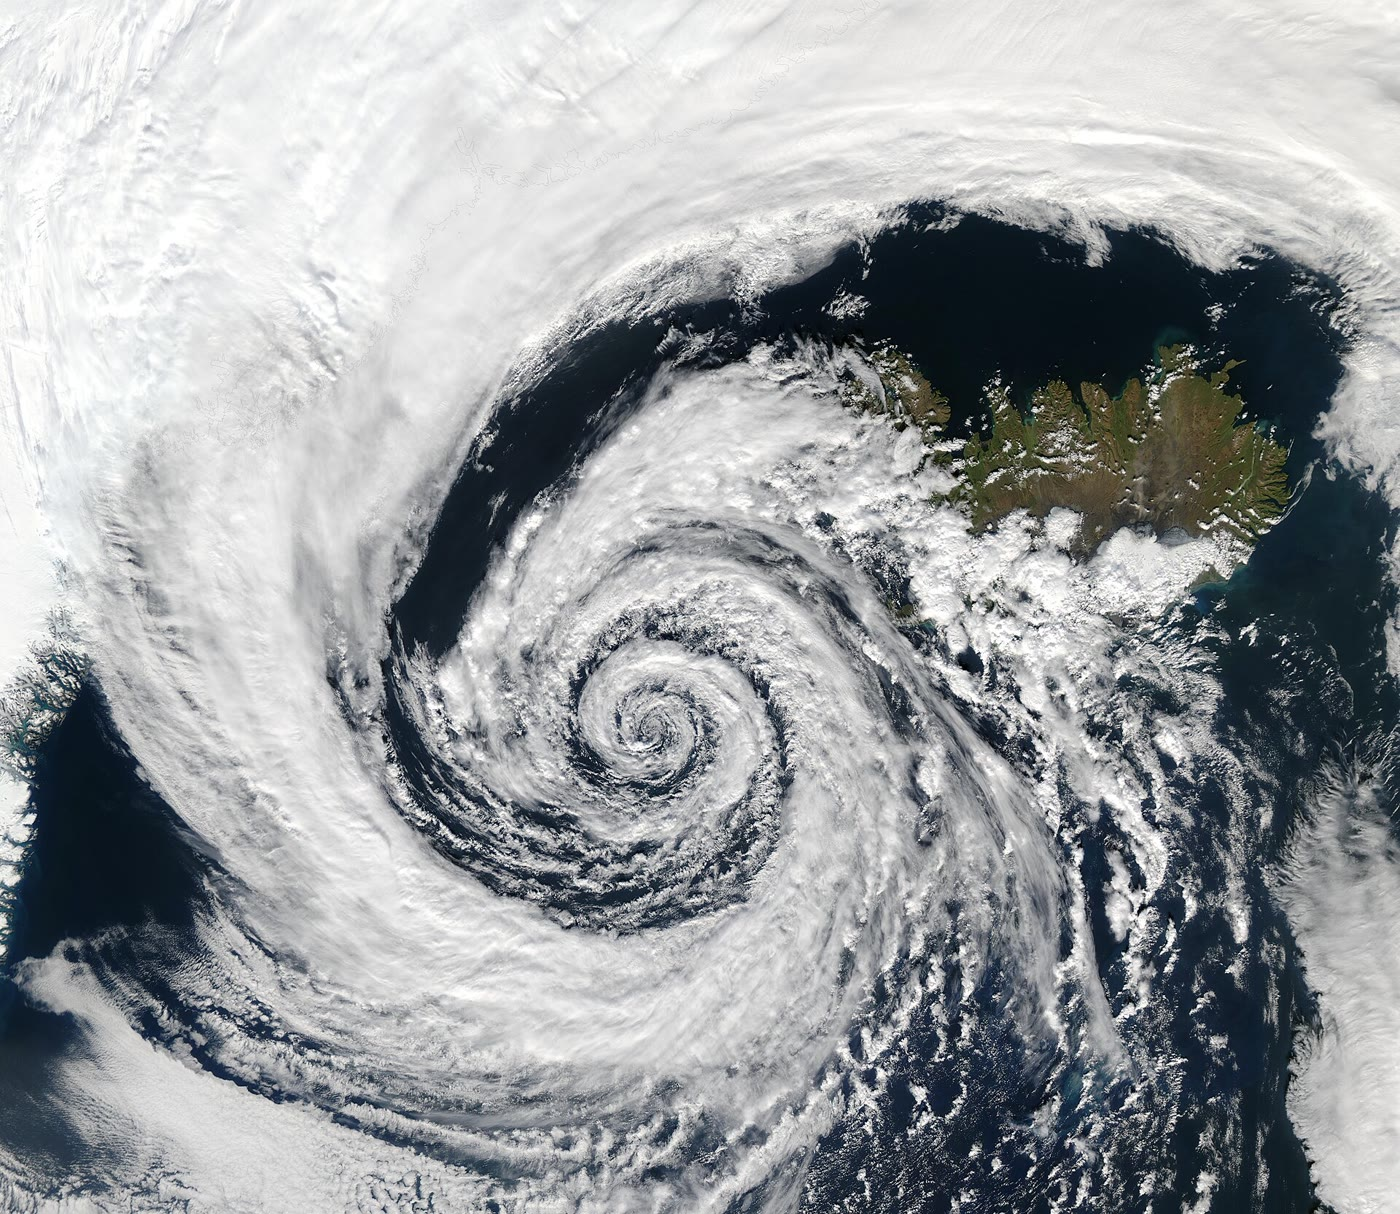
\includegraphics[width=0.58\linewidth]{images/book4/b2-22-iceland-low.jpg}
\par\smallskip{\small Une dépression profonde au large de la côte sud-ouest de l'Islande, le 4 septembre 2003, vue par
l'instrument MODIS du satellite Aqua de la NASA : les bandes nuageuses s'enroulent vers le centre. (NASA
Goddard Space Flight Center, MODIS Rapid Response Team, Jacques Descloitres, domaine public, via
Wikimedia Commons.)}
\end{omfigure}

\section{Courants-jets et ondes de Rossby}\label{sec:b2:weather-systems:rossby}

Les cyclones ne sont pas dispersés au hasard. Le courant-jet polaire, cœur rapide des vents d'ouest au-dessus
du front polaire, suit la position et le déplacement des anticyclones et des dépressions des moyennes
latitudes~; il est plus rapide le long de ses maxima de vent, les tronçons où sa vitesse culmine, et il
ne fait pas le tour du pôle en anneau : il serpente.
% ledger: nws4:polar-front, nws4:jet-streak

\begin{definition}[Onde de Rossby~; talweg et dorsale d'altitude]\label{def:b2:weather-systems:rossby}
Une \emph{onde de Rossby}\index{onde de Rossby} est une onde du courant d'ouest de la haute troposphère,
une suite de talwegs et de dorsales longs de milliers de kilomètres, à grande amplitude nord--sud.
Un \emph{talweg d'altitude}\index{talweg d'altitude} est une région allongée de pression relativement basse
dans une telle onde, où l'écoulement se courbe vers l'équateur ; une \emph{dorsale d'altitude}\index{dorsale d'altitude}
est une région allongée de pression relativement haute, où il se courbe
vers le pôle.
\end{definition}
% ledger: nws4:rossby

Les \omterm{def:b2:weather-systems:rossby}{ondes de Rossby} existent parce que le paramètre de Coriolis croît vers le pôle. Un air poussé vers le pôle
trouve un $f$ plus grand et, en conservant sa vorticité absolue, revient vers l'équateur ; un air poussé vers l'équateur
revient vers le pôle. Le taux de croissance de $f$ vers le nord,
$\beta = \mathrm{d}f/\mathrm{d}y = 2\Omega\cos\varphi/a$ avec $a$ le rayon de la Terre, règle leur vitesse.
Le volume de troisième année démontre, à partir de la conservation de la vorticité, la vitesse de phase d'une
onde de longueur d'onde $\lambda$ dans un vent d'ouest uniforme $U$~:
\[
  c = U - \frac{\beta}{k^2}, \qquad k = \frac{2\pi}{\lambda} .
\]
Admettons-le ici. Par rapport à l'air, toute \omterm{def:b2:weather-systems:rossby}{onde de Rossby} se déplace vers l'ouest, et d'autant plus vite que l'onde est longue~;
le vent l'emporte vers l'est. Les ondes courtes sont emportées vers l'est presque à la vitesse du vent,
les longues dérivent lentement, restent immobiles ou se déplacent même vers l'ouest.
% ledger: earth:Trot, earth:Rmean

\begin{example}[Trois ondes à \ang{45}~N]\label{ex:b2:weather-systems:rossby}
Avec $\Omega = \qty{7.292e-5}{s^{-1}}$ (un jour sidéral de \qty{23.9345}{h}) et $a =
\qty{6371}{km}$, $\beta = \qty{1.62e-11}{m^{-1}.s^{-1}}$ à \ang{45}~N. Dans un vent d'ouest de
\qty{15}{m/s}, une onde de \qty{4000}{km} a $\beta/k^2 = \qty{6.6}{m/s}$ et se déplace vers l'est à
\qty{8.4}{m/s}~; une de \qty{6000}{km} a $\beta/k^2 = \qty{14.8}{m/s}$ et tient à peine en place, à
\qty{0.2}{m/s}~; une de \qty{8000}{km} se déplace vers l'ouest à \qty{11.2}{m/s}.
\end{example}
% ledger: earth:Trot, earth:Rmean

Les talwegs des ondes longues se déplacent lentement et durent longtemps ; les ondes courtes qui les traversent,
les talwegs d'ondes courtes, provoquent une ascendance d'air devant eux, sur leur flanc est, là où la pression de surface baisse
et où naissent des dépressions. Un talweg dont l'axe s'incline du sud-est vers le nord-ouest est souvent le signe
d'un système en formation ou en intensification.
% ledger: nws4:rossby

\begin{omfigure}
\centering
\begin{tikzpicture}[font=\scriptsize, >=Stealth]
\foreach \lat/\pa in {30/-72, 45/-72, 60/-108} {
  \pgfmathsetmacro{\r}{6.0*tan((90-\lat)/2)}
  \draw[black!25] (0,0) circle (\r);
  \node[black!50, fill=white, inner sep=1pt] at (\pa:\r) {\ang{\lat} N};
}
\fill (0,0) circle (0.6mm);
\node[anchor=north, black!60] at (0,-0.08) {Pôle Nord};
\draw[ocBlue, very thick, smooth, samples=241, domain=0:360]
  plot ({6.0*tan((90-(47+11*cos(5*\x)))/2)*cos(\x)}, {6.0*tan((90-(47+11*cos(5*\x)))/2)*sin(\x)});
\foreach \a in {18, 90, 162, 234, 306} {
  \pgfmathsetmacro{\ra}{6.0*tan((90-(47+11*cos(5*\a)))/2)}
  \pgfmathsetmacro{\rb}{6.0*tan((90-(47+11*cos(5*(\a+2))))/2)}
  \draw[ocBlue, very thick, -{Stealth[length=2.6mm]}] (\a:\ra) -- (\a+2:\rb);
}
\pgfmathsetmacro{\rt}{6.0*tan((90-36)/2)}
\node[anchor=216, ocRed!80!black, inner sep=2pt] at (36:\rt) {talweg};
\node[anchor=0, ocRed!80!black, inner sep=2pt] at (180:\rt) {talweg};
\pgfmathsetmacro{\rr}{6.0*tan((90-58)/2)}
\node[anchor=72, ocRed!80!black, inner sep=3pt] at (72:\rr) {dorsale};
\end{tikzpicture}
\par\smallskip{\small \omterm{def:b2:weather-systems:rossby}{Ondes de Rossby} du courant-jet vues d'au-dessus du pôle Nord (schéma)~:
cinq ondes autour de l'hémisphère, des talwegs qui descendent vers l'équateur et des dorsales qui remontent vers le pôle. Le jet
circule vers l'est, dans le sens antihoraire vu d'au-dessus du pôle (flèches). Les cercles de latitude
sont tracés comme sur une carte polaire stéréographique.}
\end{omfigure}
% ledger: nws4:rossby

Parfois la configuration cesse entièrement de se déplacer.

\begin{definition}[Blocage atmosphérique]\label{def:b2:weather-systems:blocking}
Le \emph{blocage atmosphérique}\index{blocage atmosphérique} est un système de haute pression vaste, persistant et presque
immobile, parfois associé à une dépression, qui interrompt l'écoulement normal vers l'est
du courant-jet. Presque toutes les méthodes de détection des blocages exigent qu'il dure au moins cinq
jours.
\end{definition}
% ledger: wang26:blocking

Un blocage détourne le courant-jet et les cyclones qui l'entourent, et maintient le même temps sur la même
région pendant des jours : les blocages apportent canicules, sécheresses, feux de forêt, vagues de froid et inondations
aux moyennes latitudes. Fin juin et début juillet 2021, un fort blocage a produit la canicule de la côte nord-ouest
du Pacifique, en Amérique du Nord, qui a causé plus de mille morts. Les processus physiques
à l'origine du blocage restent mal compris, et les modèles numériques peinent à reproduire
la fréquence des blocages et leur durée.
% ledger: wang26:blocking, wang26:gaps

\section{Cyclones tropicaux}\label{sec:b2:weather-systems:tropical}

Les cyclones tropicaux n'ont ni fronts ni contraste de température pour s'alimenter. Ils puisent leur énergie dans
l'océan chaud, par la chaleur latente de l'eau qu'ils évaporent, comme on l'a mesuré au \cref{ch:b2:atmospheric-thermodynamics}.
Six conditions favorisent leur formation~: une eau de mer d'au moins \qty{26.5}{\celsius}
sur une profondeur de l'ordre de \qty{50}{m} ; une atmosphère qui se refroidit assez vite avec l'altitude pour être
instable à la convection humide ; une troposphère moyenne humide, vers \qty{5}{km} ; une distance d'au moins environ
\qty{500}{km} de l'équateur, de sorte que la force de Coriolis puisse maintenir la dépression en
équilibre ; une perturbation préexistante près de la surface ; et un faible cisaillement vertical du vent, inférieur à environ
\qty{10}{m/s} entre la surface et la haute troposphère. Ces conditions sont nécessaires mais non
suffisantes~: beaucoup de perturbations qui les rencontrent ne se développent jamais.
% ledger: aoml:tc-genesis

Une fois formé, un cyclone tropical est une machine thermique. L'air s'enroule vers le centre au-dessus de la mer,
à température presque constante, en prenant chaleur et humidité à l'océan ; dans le mur de l'œil il s'élève
de façon adiabatique ; dans l'échappement près de la tropopause, il perd de la chaleur par rayonnement à basse
température, presque constante ; puis il redescend loin du centre, bouclant un cycle qui ressemble à celui
de Carnot. Le travail du cycle entretient les vents contre le frottement à la
surface de la mer.
% ledger: gilford21:pi

\begin{omfigure}
\centering
\begin{tikzpicture}[font=\scriptsize, >=Stealth, x=1cm, y=1cm]
% sea and axis
\fill[ocBlue!12] (0,-0.35) rectangle (12.5,0);
\draw[thick, ocBlue!70!black] (0,0) -- (12.5,0);
\node[anchor=north west, ocBlue!70!black] at (8.6,-0.02) {mer chaude, $T_s$};
\draw[dashed, black!50] (0,-0.35) -- (0,4.9);
\node[anchor=south, black!60] at (0,4.9) {centre};
% eyewall cloud and outflow cloud
\fill[black!14, draw=black!40] (0.9,0.25) .. controls (0.7,1.8) and (0.75,3.3) .. (0.95,4.2)
  .. controls (3.5,4.55) and (7.0,4.45) .. (9.5,4.2) .. controls (7.0,3.9) and (3.6,3.85)
  .. (2.1,3.7) .. controls (1.95,2.6) and (1.9,1.4) .. (2.0,0.25) -- cycle;
\node[black!60] at (0.45,2.0) [rotate=90] {œil};
\draw[black!50] (1.9,1.1) -- (2.45,1.1) node[anchor=west, black!70] {nuage du mur de l'œil};
% the cycle
\draw[->, very thick, ocRed] (11.4,0.3) -- (2.3,0.3);
\draw[->, very thick, ocRed] (1.45,0.45) .. controls (1.4,1.6) and (1.45,3.0) .. (1.75,4.0);
\draw[->, very thick, ocBlue] (2.2,4.25) -- (11.2,4.25);
\draw[->, very thick, ocBlue] (11.6,4.05) .. controls (11.75,2.8) and (11.75,1.5) .. (11.6,0.45);
\fill (11.6,0.3) circle (0.7mm) node[right=2pt] {A};
\fill (1.45,0.3) circle (0.7mm) node[left=2pt] {B};
\fill (1.8,4.25) circle (0.7mm) node[above left=1pt] {C};
\fill (11.6,4.25) circle (0.7mm) node[above right=1pt] {D};
\node[anchor=south, align=center] at (6.5,0.35) {A$\to$B~: afflux sur la mer à environ $T_s$,
  prélevant chaleur et humidité};
\node[anchor=west, align=left] at (2.25,2.3) {B$\to$C~: montée dans le mur de l'œil,\\sans
  échange de chaleur (adiabatique humide)};
\node[anchor=south, align=center] at (6.5,4.62) {C$\to$D~: échappement près de la tropopause à environ
  $T_o$, perte de chaleur par rayonnement};
\node[anchor=east, align=right] at (11.45,2.3) {D$\to$A~: descente loin\\du centre};
\end{tikzpicture}
\par\smallskip{\small Le moteur thermique d'un cyclone tropical, coupe verticale depuis le centre
vers l'extérieur (schéma, non à l'échelle)~: la chaleur est prélevée à la température de la surface de la mer
(A$\to$B) et restituée à la température bien plus basse de l'échappement (C$\to$D), comme dans un cycle de
Carnot.}
\end{omfigure}
% ledger: gilford21:pi

\begin{proposition}[Intensité potentielle]\label{prop:b2:weather-systems:pi}
\index{intensité potentielle}
L'\emph{\omterm{prop:b2:weather-systems:pi}{intensité potentielle}} d'un cyclone tropical, la vitesse maximale du vent près de la surface que
l'océan et l'atmosphère qui l'entourent peuvent entretenir, est approximativement donnée par
\[
  V_{\max}^2 = \frac{C_k}{C_D}\,\frac{T_s - T_o}{T_o}\,\bigl(h_o^* - h^*\bigr),
\]
où $T_s$ est la température de la surface de la mer, $T_o$ celle de l'échappement, $C_k/C_D$
le rapport des coefficients d'échange d'enthalpie et de quantité de mouvement entre la mer et l'air,
généralement pris égal à 0.9, et $h_o^* - h^*$ l'excès de $c_pT + gz + Lq$ à saturation à la surface de la mer
sur sa valeur à saturation dans l'air au-dessus de la couche limite (admis).
\end{proposition}
% ledger: gilford21:pi

La fraction $(T_s - T_o)/T_o$ n'est pas le rendement de Carnot $(T_s - T_o)/T_s$ des
volumes de physique~: elle est plus grande, du facteur $T_s/T_o$, car le frottement qui dissipe le travail réchauffe
l'air entrant près de la surface de la mer, et cette chaleur est réutilisée par le moteur. Le dernier
facteur est le carburant. Dans une atmosphère tropicale dont la température suit l'\omterm{def:b2:atmospheric-thermodynamics:moist-adiabat}{adiabatique humide} de son air
de couche limite, $h^*$ est la valeur de $c_pT + gz + Lq$ dans cet air, et $h_o^* - h^*$
mesure l'écart à la saturation, à la température de la mer, de l'air au-dessus de la mer~:
\[
  h_o^* - h^* \approx c_p\,(T_s - T_a) + L\,(q_s^* - q_a),
\]
avec $T_a$ et $q_a$ la température et l'\omterm{def:b2:atmospheric-thermodynamics:moist-air}{humidité spécifique} de l'air près de la surface, et
$q_s^*$ l'\omterm{def:b2:atmospheric-thermodynamics:moist-air}{humidité spécifique} à saturation à la température de surface de la mer.
% ledger: gilford21:pi

\begin{example}[Une intensité potentielle]\label{ex:b2:weather-systems:pi}
Au-dessus d'une mer à \qty{29}{\celsius}, l'air à \qty{1015}{hPa} est à \qty{28}{\celsius} avec une
humidité relative de \qty{80}{\percent}, et l'échappement est à \qty{200}{K}, une moyenne annuelle typique des océans
tropicaux chauds. D'après les \cref{prop:b2:atmospheric-thermodynamics:es,prop:b2:atmospheric-thermodynamics:humidity},
$e_s(\qty{29}{\celsius}) = \qty{41.0}{hPa}$, donc $q_s^* = \qty{25.5}{g/kg}$, et l'air, avec
$e = 0.8 \times \qty{38.7}{hPa}$, a $q_a = \qty{19.2}{g/kg}$. Alors $h_o^* - h^* = 1004.5 \times
1 + 2.501 \times 10^6 \times 0.0063 = \qty{16.8}{kJ/kg}$, le facteur $(T_s - T_o)/T_o$ vaut
$(302.15 - 200)/200 = 0.511$, et $V_{\max} = \sqrt{0.9 \times 0.511 \times 16\,800} =
\qty{88}{m/s}$.
\end{example}
% ledger: gilford21:pi

Les tempêtes les plus fortes approchent de telles valeurs : le haut de l'échelle de Saffir--Simpson, la catégorie
5, commence à \qty{70}{m/s}, et cinq tempêtes récentes ont dépassé \qty{86}{m/s}. La plupart des tempêtes
n'atteignent que rarement leur \omterm{prop:b2:weather-systems:pi}{intensité potentielle}~: les tempêtes réelles sont rarement dans l'état stationnaire que suppose
la théorie, qui néglige le cisaillement vertical du vent, l'air sec aspiré dans la tempête et la subsidence de l'air
qui l'entoure, autant de facteurs qui affaiblissent une tempête.
% ledger: wk24:scale, gilford21:limits, aoml:tc-weaken

\begin{omfigure}
\centering
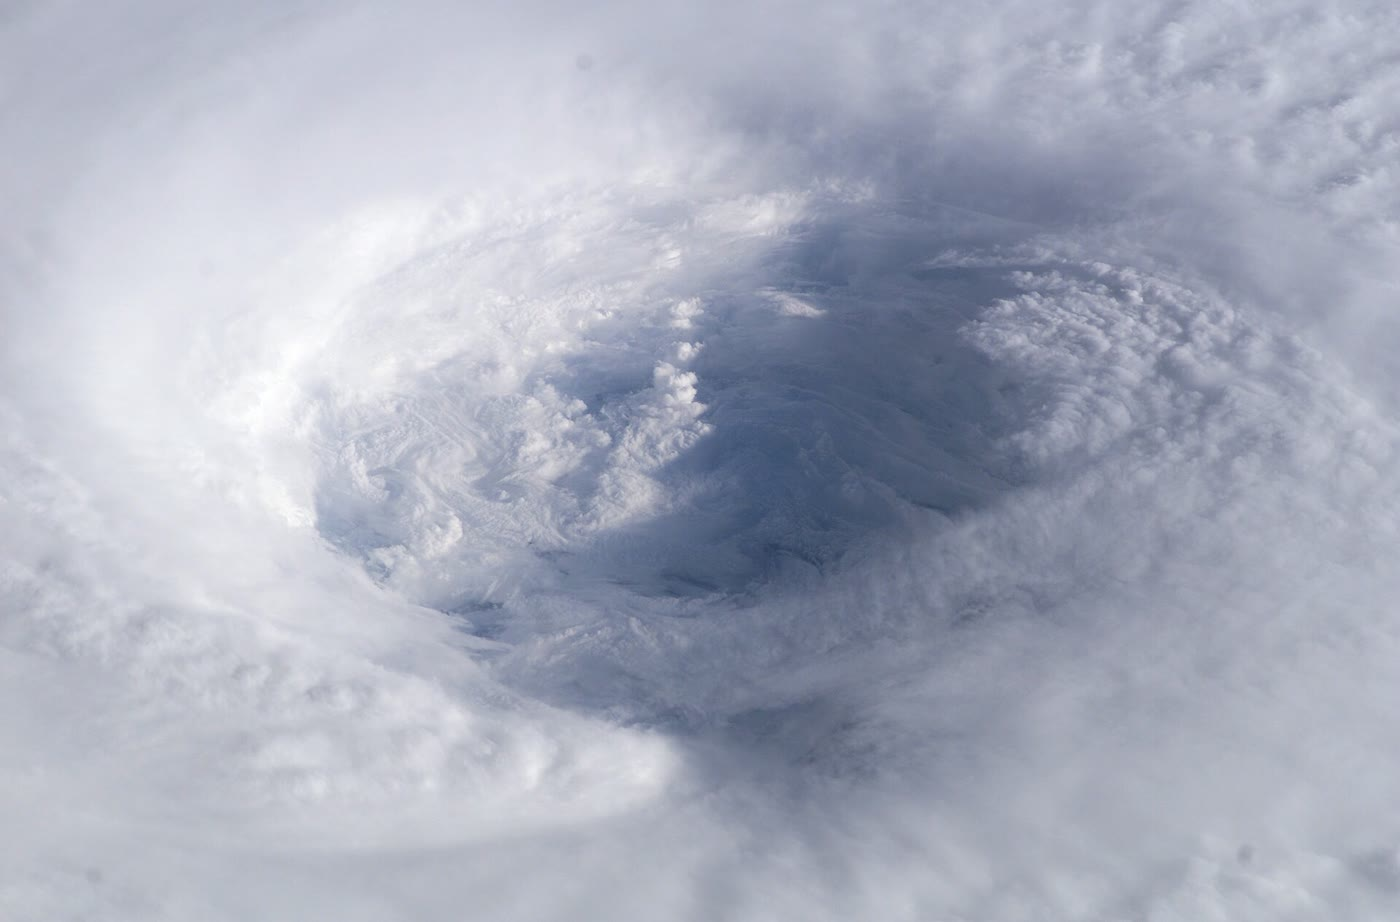
\includegraphics[width=0.62\linewidth]{images/book4/b2-22-isabel-eye.jpg}
\par\smallskip{\small L'œil de l'ouragan Isabel, le 13 septembre 2003, photographié depuis la Station spatiale
internationale : le mur de l'œil tombe comme un stade jusqu'aux nuages bas de l'œil.
(Astronaute de la NASA Ed Lu, domaine public, via Wikimedia Commons.)}
\end{omfigure}

\section{Prévision numérique du temps}\label{sec:b2:weather-systems:nwp}

\begin{definition}[Prévision numérique du temps~; assimilation de données~; prévision d'ensemble~; limite de prévisibilité]\label{def:b2:weather-systems:nwp}
La \emph{prévision numérique du temps}\index{prévision numérique du temps} est la prévision par ordinateur : les équations
qui gouvernent le mouvement, l'énergie et l'eau de l'atmosphère sont intégrées dans le temps à partir de son état
observé. L'\emph{assimilation de données}\index{assimilation de données} combine les dernières observations à une
prévision à courte échéance issue d'observations antérieures, pour obtenir la meilleure estimation de l'état présent,
l'analyse, à partir de laquelle part la prévision. Une \emph{prévision d'ensemble}\index{prévision d'ensemble} est un
ensemble de prévisions lancées à partir d'états initiaux légèrement différents, et avec des versions légèrement différentes
du modèle, pour montrer l'éventail des temps possibles et leur vraisemblance. La \emph{limite de
prévisibilité}\index{limite de prévisibilité} est le temps au-delà duquel une prévision de l'état du temps ne vaut
pas mieux qu'une estimation climatique, parce que les erreurs de
l'état initial sont devenues aussi grandes que les
écarts entre deux états quelconques de l'atmosphère.
\end{definition}
% ledger: nws4:nwp, ecmwf4:da, ecmwf4:ens-fs, krish19:predictability

La première prévision numérique fut calculée en 1950 sur l'ENIAC, l'un des premiers
ordinateurs électroniques. Un modèle global d'aujourd'hui découpe l'atmosphère en une grille de mailles de quelques kilomètres
de côté et part d'une analyse qui mêle les observations des stations météorologiques, des avions,
des \omterm{def:b2:atmospheric-thermodynamics:sounding}{radiosondages}, des navires, des bouées et, surtout, des satellites, qui apportent la plus grande part
de l'habileté des prévisions globales. Dans un grand centre de prévision, l'ensemble
compte 51 membres, une simulation de contrôle et 50 perturbées, à une résolution d'environ \qty{9}{km}, lancé
deux fois par jour jusqu'à 15 jours à l'avance.
% ledger: krish19:predictability, ecmwf4:da, ecmwf4:ens

Pourquoi perturber une prévision qui pourrait partir de la meilleure analyse~? Parce que l'atmosphère est
chaotique, sensible à son état initial. Un système de trois variables publié en 1963 le montre
à la plus petite échelle.

\begin{proposition}[Le système de Lorenz]\label{prop:b2:weather-systems:lorenz}
Le système
\[
  \dot x = \sigma(y - x), \qquad \dot y = x(r - z) - y, \qquad \dot z = xy - bz,
\]
avec $\sigma = 10$, $r = 28$ et $b = 8/3$, possède les propriétés suivantes.
\begin{enumerate}
  \item Ses points fixes sont l'origine et $C_\pm = \bigl(\pm\sqrt{b(r - 1)}, \pm\sqrt{b(r - 1)},
        r - 1\bigr) = (\pm 8.49, \pm 8.49, 27)$.
  \item Chaque volume de son espace des phases décroît comme $\mathrm{e}^{-(\sigma + 1 + b)t}$~: ses
        trajectoires aboutissent sur un ensemble de volume nul, l'attracteur.
  \item Sur l'attracteur, deux trajectoires partant à une petite distance $\delta_0$ l'une de l'autre se séparent,
        en moyenne, selon $\delta(t) \approx \delta_0\,\mathrm{e}^{\lambda t}$, avec $\lambda =
        0.906$, jusqu'à ce que $\delta$ atteigne la taille de l'attracteur (calculé, admis). Les petites
        erreurs doublent tous les $\ln 2/\lambda = 0.77$ unité de temps.
\end{enumerate}
\end{proposition}
% ledger: nolitia22:lorenz

\begin{proof}[Démonstration des points 1 et 2]
À un point fixe, $y = x$ d'après la première équation ; la troisième donne $z = x^2/b$ ; la deuxième
devient $x(r - 1 - x^2/b) = 0$, donc $x = 0$ ou $x^2 = b(r - 1) = 72$. La divergence du champ de vecteurs vaut
$\partial_x\dot x + \partial_y\dot y + \partial_z\dot z = -\sigma - 1 - b$, une constante, par le théorème
de la divergence : un volume $V$ transporté par l'écoulement obéit à $\dot V =
-(\sigma + 1 + b)V$.
\end{proof}

Les figures montrent ce que dit la proposition. Deux trajectoires partant à \num{e-5} l'une de l'autre se suivent pendant
une quinzaine d'unités de temps, puis se séparent pour de bon : chacune ressemble encore à une trajectoire plausible
du système, mais ce ne sont plus la même trajectoire. En moyenne sur 200 couples de trajectoires lancées à \num{e-8} l'une de l'autre,
la distance croît exponentiellement au taux $\lambda$, une droite en échelle logarithmique,
jusqu'à saturer à la taille de l'attracteur. Quelle que soit l'erreur initiale, elle atteint cette taille : une erreur
initiale plus petite ne fait que retarder le moment de
$\ln 10/\lambda = 2.5$ unités de temps pour chaque division par dix.
% ledger: nolitia22:lorenz

\begin{omfigure}
\centering
% figdata/bachelor-2/weather.py parts traj, butterfly
\begin{tikzpicture}
\begin{groupplot}[group style={group size=2 by 1, horizontal sep=1.5cm},
  tick label style={font=\scriptsize}, label style={font=\small}]
\nextgroupplot[width=0.58\linewidth, height=5.0cm, xmin=0, xmax=30, ymin=-22, ymax=22,
  xlabel={temps}, ylabel={$x$}, legend style={font=\scriptsize, at={(0.5,1.02)},
  anchor=south, draw=none, legend columns=2, /tikz/every even column/.append style={column
  sep=0.4cm}}, legend cell align=left]
\addplot[ocBlue, thin] table[x=t, y=x1] {figdata/out/bachelor-2-weather-traj.dat};
\addlegendentry{trajectoire 1}
\addplot[ocRed, thin, densely dashed] table[x=t, y=x2] {figdata/out/bachelor-2-weather-traj.dat};
\addlegendentry{trajectoire 2, lancée à \num{e-5} de la première}
\nextgroupplot[width=0.4\linewidth, height=5.0cm, xmin=-22, xmax=22, ymin=0, ymax=52,
  xlabel={$x$}, ylabel={$z$}]
\addplot[black!70, very thin] table[x=x, y=z] {figdata/out/bachelor-2-weather-butterfly.dat};
\addplot[only marks, mark=*, mark size=1.3pt, ocRed] coordinates {(8.485,27) (-8.485,27)};
\end{groupplot}
\end{tikzpicture}
\par\smallskip{\small Le système de Lorenz ($\sigma = 10$, $r = 28$, $b = 8/3$), intégré par la
méthode de Runge--Kutta avec un pas de temps de 0.01. À gauche : deux trajectoires partant à \num{e-5} l'une de l'autre en $x$
sur l'attracteur. À droite : une trajectoire sur 40 unités de temps, vue selon $y$, avec les points fixes
$C_\pm$ (en rouge).}
\end{omfigure}
% ledger: nolitia22:lorenz

\begin{omfigure}
\centering
% figdata/bachelor-2/weather.py part growth
\begin{tikzpicture}
\begin{axis}[width=0.72\linewidth, height=5.6cm, xmin=0, xmax=30, ymode=log, ymin=1e-9,
  ymax=1e3, ytick={1e-9,1e-7,1e-5,1e-3,1e-1,1e1,1e3}, xlabel={temps}, ylabel={distance entre les trajectoires}, tick label style={font=\scriptsize},
  label style={font=\small}, legend style={font=\scriptsize, at={(0.02,0.98)}, anchor=north west,
  draw=none, fill=none}, legend cell align=left, unbounded coords=discard, grid=major,
  grid style={black!8}]
\addplot[ocBlue, line width=1.6pt, opacity=0.55] table[x=t, y expr=10^\thisrow{log10d}]
  {figdata/out/bachelor-2-weather-growth.dat};
\addlegendentry{moyenne de 200 couples (géométrique)}
\addplot[black, densely dashed, thin] table[x=t, y expr=10^\thisrow{fit}]
  {figdata/out/bachelor-2-weather-growth.dat};
\addlegendentry{exponentielle ajustée, $t = 2$ à 16}
\end{axis}
\end{tikzpicture}
\par\smallskip{\small Croissance de la distance entre couples de trajectoires du système de Lorenz lancées à
\num{e-8} l'une de l'autre. La droite ajustée est multipliée par dix tous les 2.57 unités de temps, soit un taux de 0.897~;
l'exposant de Lyapunov le plus grand, calculé en renormalisant un seul couple sur 2000 unités de temps, vaut
0.909, contre 0.906 publié. La croissance s'arrête à la taille de l'attracteur.}
\end{omfigure}
% ledger: nolitia22:lorenz

L'atmosphère se comporte de la même façon, avec bien plus de variables et des erreurs qui croissent
à des taux différents selon les échelles. D'après les prévisions des années 1980, on a constaté que les petites erreurs
doublaient en environ 2.4 jours, et que la prévision fiable de l'état du temps s'arrête vers une dizaine de jours.
Des expériences qui réduisent l'incertitude actuelle sur l'état initial, avec un modèle supposé parfait,
montrent que des conditions initiales parfaites n'ajouteraient que quatre à cinq jours, et qu'une réduction
de \qty{90}{\percent} en donne déjà presque tout : à mesure que les erreurs diminuent, elles croissent plus vite,
par le dégagement de chaleur latente dans la convection, à des échelles plus petites que celles que la prévision
ne peut résoudre. La \omterm{def:b2:weather-systems:nwp}{limite de prévisibilité} des moyennes latitudes se situe vers deux semaines. Les prévisions
gagnent environ un jour par décennie, parce que de meilleures observations, l'assimilation et les modèles les rapprochent
de cette limite ; elles ne peuvent la franchir.
% ledger: krish19:predictability, selz22:limit, bauer:day-per-decade

L'ensemble en fait un outil. Ses membres partent d'analyses qui diffèrent à peu près autant que l'analyse elle-même
est incertaine ; tant qu'ils s'accordent, la prévision est nette ; quand ils se dispersent, la prévision doit le dire
et donne des probabilités.
Une prévision est dite fiable lorsque les événements qu'elle annonce avec une probabilité
de \qty{70}{\percent} se produisent dans \qty{70}{\percent} des cas.
% ledger: ecmwf4:ens-fs

\begin{inthelab}[Une journée dans un centre de prévision]
\begin{minipage}[t]{0.54\linewidth}\vspace{0pt}
Dans un centre de prévision mondial, la journée s'organise autour de deux échéances, 00 et 12 UTC. Les observations valables
autour de chacune arrivent par millions, des satellites, des \omterm{def:b2:atmospheric-thermodynamics:sounding}{radiosondages}, des avions, des navires, des bouées
et des stations météorologiques ; l'\omterm{def:b2:weather-systems:nwp}{assimilation de données} les combine à la prévision courte précédente pour
produire l'analyse. Les modèles partent de celle-ci, l'ensemble aussi, et les prévisions parviennent à leurs utilisateurs
plusieurs heures plus tard, une fois que les superordinateurs ont calculé les 15 jours à venir. Les prévisionnistes
comparent alors les simulations, les confrontent aux dernières observations et aux images satellite, suivent les
cyclones et les fronts, et transforment les probabilités de l'ensemble en avertissements et en
prévisions.
\end{minipage}\hfill
\begin{minipage}[t]{0.42\linewidth}\vspace{0pt}
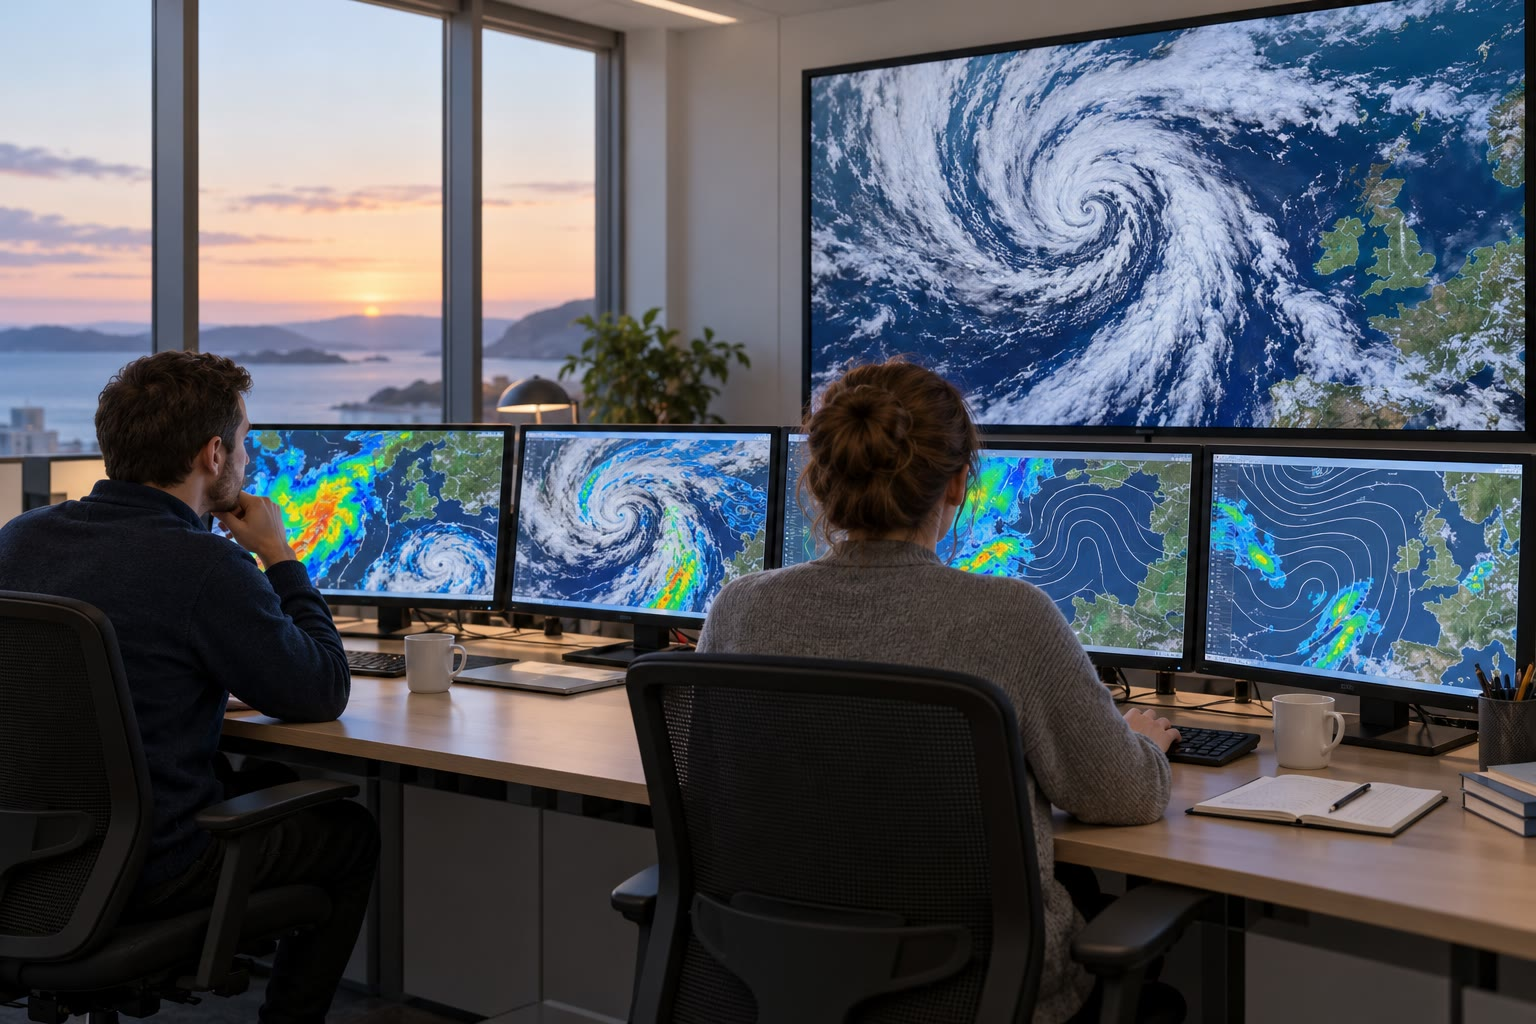
\includegraphics[width=\linewidth]{images/book4/ai/b2-forecast-office.jpg}

{\scriptsize Prévisionnistes au travail devant des images satellite et des cartes de modèles
(Illustration générée par IA.)}
\end{minipage}
% ledger: ecmwf4:ens, ecmwf4:da, mo:how-forecasts
\end{inthelab}

\section*{Exercices}\label{sec:b2:weather-systems:exercises}

Données pour les exercices, sauf indication contraire~: $\Omega = \qty{7.292e-5}{s^{-1}}$, $a =
\qty{6371}{km}$, $g = \qty{9.81}{m.s^{-2}}$, $c_p = \qty{1004.5}{J.kg^{-1}.K^{-1}}$, $L =
\qty{2.501e6}{J/kg}$, et la \omterm{def:b2:atmospheric-thermodynamics:moist-air}{pression de vapeur} saturante des exercices du
\cref{ch:b2:atmospheric-thermodynamics}.
% ledger: earth:Trot, earth:Rmean

\begin{exercise}[$\star$]\label{exo:b2:weather-systems:1}
À \ang{50}~N, un front froid sépare de l'air à \qty{275}{K} d'air à \qty{281}{K}, et le vent
le long de lui varie de \qty{15}{m/s}. (a) Calculer $f$. (b) Calculer la pente de la \omterm{def:b2:weather-systems:fronts}{surface frontale},
sous la forme 1 sur $N$. (c) À quelle distance derrière le front, au sol, la \omterm{def:b2:weather-systems:fronts}{surface frontale} atteint-elle
\qty{1}{km}~? (d) Que devient la pente si le contraste de température double, pour le même
changement de vent~?
\end{exercise}

\begin{exercise}[$\star$]\label{exo:b2:weather-systems:2}
Une \omterm{def:b2:weather-systems:fronts}{surface frontale} chaude monte à 1 sur 150 et le front se déplace à \qty{25}{km/h}. (a) À quelle distance
en avant du front, au sol, la \omterm{def:b2:weather-systems:fronts}{surface frontale} se trouve-t-elle à \qty{6}{km} d'altitude~? (b) Un observateur y voit
se former des nuages élevés : combien de temps après le front atteint-il l'observateur~? (c) Décrire la succession
des nuages que voit l'observateur pendant ce temps.
\end{exercise}
% ledger: ucar:warm-front

\begin{exercise}[$\star$]\label{exo:b2:weather-systems:3}
Sur une carte de l'hémisphère Nord, (a) une ligne à triangles bleus sur son côté sud-est part vers le sud-ouest
depuis une dépression ; (b) une ligne à demi-cercles rouges sur son côté nord part vers l'est depuis la même dépression ; (c) une
ligne violette portant les deux symboles relie une autre dépression à un point d'où partent deux autres fronts ; (d) une
ligne alterne triangles bleus sur son côté sud et demi-cercles rouges sur son côté nord. Nommer chaque front, dire où se trouve
l'air froid et dans quel sens se déplace chacun.
\end{exercise}
% ledger: ucar4:stationary-occluded, nws4:occluded

\begin{exercise}[$\star$]\label{exo:b2:weather-systems:4}
À \ang{45}~N, dans un vent d'ouest de \qty{12}{m/s}~: (a) calculer $\beta$. (b) Calculer la vitesse de phase
des ondes de \qty{4000}{km} et de \qty{8000}{km}. (c) Dans quel sens se déplace chacune, et sur quelle distance en un
jour~?
\end{exercise}

\begin{exercise}[$\star\star$]\label{exo:b2:weather-systems:5}
(a) Montrer qu'une \omterm{def:b2:weather-systems:rossby}{onde de Rossby} reste immobile dans un vent d'ouest $U$ lorsque $\lambda = 2\pi\sqrt{U/\beta}$.
(b) Calculer cette longueur d'onde à \ang{45}~N pour $U = \qty{12}{m/s}$. (c) Combien de telles ondes tiennent autour
du cercle de latitude~? (d) Pourquoi un vent d'ouest plus fort favoriserait-il des ondes stationnaires moins nombreuses et plus longues~?
\end{exercise}

\begin{exercise}[$\star\star$]\label{exo:b2:weather-systems:6}
Pour le système de Lorenz~: (a) vérifier que $C_+$ est un point fixe en calculant les trois dérivées
en ce point. (b) De quel facteur un petit volume de l'espace des phases diminue-t-il en une unité de temps~? (c) Pourquoi
cela n'empêche-t-il pas deux trajectoires voisines de se séparer~?
\end{exercise}

\begin{exercise}[$\star\star$]\label{exo:b2:weather-systems:7}
Prendre $\lambda = 0.906$ pour le système de Lorenz et un attracteur de taille 10. (a) Calculer le
temps de doublement des petites erreurs. (b) Combien de temps une erreur de \num{e-8} met-elle à atteindre la taille de
l'attracteur~? (c) De combien une erreur initiale mille fois plus petite retarde-t-elle ce moment~? Quelle fraction du temps trouvé en
(b) cela représente-t-il~?
\end{exercise}
% ledger: nolitia22:lorenz

\begin{exercise}[$\star\star$]\label{exo:b2:weather-systems:8}
Une mer à \qty{303}{K} a un échappement à \qty{195}{K} ; le déséquilibre vaut $h_o^* - h^* =
\qty{15}{kJ/kg}$ et $C_k/C_D = 0.9$. (a) Calculer l'\omterm{prop:b2:weather-systems:pi}{intensité potentielle}. (b) La comparer au seuil
de la catégorie 5 et aux tempêtes récentes les plus rapides. (c) Pourquoi la plupart des tempêtes
n'atteignent-elles pas cette valeur~?
\end{exercise}
% ledger: gilford21:pi, wk24:scale

\begin{exercise}[$\star\star$]\label{exo:b2:weather-systems:9}
Pour la tempête de l'\cref{exo:b2:weather-systems:8} : (a) calculer le rendement de Carnot d'un moteur
fonctionnant entre la surface de la mer et l'échappement. (b) Calculer le facteur $(T_s - T_o)/T_o$ de
la \cref{prop:b2:weather-systems:pi} et le rapport des deux. (c) Expliquer la différence.
\end{exercise}
% ledger: gilford21:pi

\begin{exercise}[$\star\star\star$]\label{exo:b2:weather-systems:10}
(a) Redémontrer la \cref{prop:b2:weather-systems:slope} en gardant les masses volumiques exactes, et montrer que
l'air froid doit se trouver dessous. (b) À travers une zone frontale large de \qty{50}{km} à \ang{45}~N, le vent
le long du front varie de \qty{10}{m/s}. Calculer la vorticité relative de la zone et la comparer à
$f$. (c) La zone est-elle cyclonique ou anticyclonique~?
\end{exercise}

\begin{exercise}[$\star\star\star$]\label{exo:b2:weather-systems:11}
Supposons que les erreurs de prévision doublent tous les 2.4 jours, partent de \qty{0.5}{K} et soient inutilisables à
\qty{6}{K}. (a) Trouver l'horizon des prévisions utiles. (b) De quel facteur l'erreur initiale doit-elle diminuer
chaque décennie pour gagner un jour par décennie, si le modèle était parfait~? (c) Des expériences montrent qu'une erreur
initiale dix fois plus petite ne gagne que 4 à 5 jours. Quel temps de doublement cela implique-t-il pour
les petites erreurs, et que dit-il de leur croissance~?
\end{exercise}
% ledger: krish19:predictability, selz22:limit, bauer:day-per-decade

\begin{exercise}[$\star\star\star$]\label{exo:b2:weather-systems:12}
Reprendre l'\cref{ex:b2:weather-systems:pi} et réchauffer la mer et l'air de \qty{1}{K}, l'humidité relative
et la température de l'échappement restant inchangées. (a) Recalculer $q_s^*$, $q_a$ et le
déséquilibre. (b) Recalculer l'\omterm{prop:b2:weather-systems:pi}{intensité potentielle}. (c) De combien, en pourcentage par kelvin,
augmente-t-elle, et quel facteur y contribue le plus~?
\end{exercise}
% ledger: gilford21:pi

\begin{problem}[{Problème du week-end --- Jusqu'où prévoir~?}]\label{pb:b2:weather-systems:1}
Une carte météorologique fictive à \ang{50}~N montre un front froid qui avance sur une ville, avec une \omterm{def:b2:weather-systems:rossby}{onde de Rossby}
dans le courant-jet au-dessus. Le problème suit le front, puis l'onde, et demande jusqu'où chacun peut être prévu. Utiliser
les données des exercices.

\medskip\noindent\textbf{Partie I --- Le front.}
À 06 UTC, le front froid est à \qty{480}{km} à l'ouest de la ville, à 12 UTC à \qty{390}{km}. Derrière lui
l'air est à \qty{277}{K}, dans le secteur chaud à \qty{285}{K}, et le vent le long du front
varie de \qty{16}{m/s} d'un côté à l'autre.
\begin{enumerate}
  \item Trouver la vitesse du front.
  \item À quelle heure atteint-il la ville~?
  \item Calculer $f$ à \ang{50}~N.
  \item Calculer la pente de la \omterm{def:b2:weather-systems:fronts}{surface frontale}.
  \item Quelle est la hauteur de la \omterm{def:b2:weather-systems:fronts}{surface frontale} au-dessus de la ville six heures après le passage du front~?
  \item Au bout de combien de temps après le passage l'air froid atteint-il \qty{1.5}{km} au-dessus de la ville~?
  \item Quel temps la ville observe-t-elle au passage du front, et comment évolue la pression~?
\end{enumerate}

\medskip\noindent\textbf{Partie II --- L'onde en altitude.}
Dans le courant-jet au-dessus, le vent d'ouest est de \qty{20}{m/s} et l'onde a une longueur d'onde de \qty{5000}{km}.
\begin{enumerate}[resume]
  \item Calculer $\beta$ à \ang{50}~N.
  \item Calculer $k$ et $\beta/k^2$.
  \item Trouver la vitesse de phase de l'onde.
  \item De quelle distance un talweg se déplace-t-il en 24 heures~?
  \item Trouver la longueur d'onde qui resterait immobile dans ce vent, et combien de telles ondes tiennent
         autour de \ang{50}~N.
  \item Où, par rapport au \omterm{def:b2:weather-systems:rossby}{talweg d'altitude}, le cyclone de surface doit-il s'approfondir~?
\end{enumerate}

\medskip\noindent\textbf{Partie III --- Une atmosphère modèle.}
Sur la figure de la croissance des erreurs du système de Lorenz, la droite ajustée passe par
environ \num{5e-7} à $t = 4$ et \num{3.9e-3} à $t = 14$.
\begin{enumerate}[resume]
  \item À partir de ces deux lectures, calculer le taux de croissance $\lambda$.
  \item Calculer le temps de doublement.
  \item Comparer avec l'exposant publié, 0.906.
  \item Pourquoi la distance cesse-t-elle de croître, vers 15~?
  \item De combien de temps plus tard une erreur dix fois plus petite atteint-elle cette taille~?
\end{enumerate}

\medskip\noindent\textbf{Partie IV --- Jusqu'où prévoir~?}
Prendre le temps de doublement de 2.4 jours trouvé pour les petites erreurs des prévisions des années 1980, une erreur
initiale de \qty{0.1}{\celsius} sur la température à un niveau donné, et une prévision qui devient inutilisable
dès que l'erreur atteint \qty{3}{\celsius}.
\begin{enumerate}[resume]
  \item Combien de doublements séparent l'erreur initiale de l'erreur qui rend la prévision inutilisable~?
  \item Combien de jours cela prend-il~?
  \item De combien de jours gagnerait-on en divisant l'erreur initiale par deux~?
  \item Avec l'estimation antérieure d'un temps de doublement de 5 jours, quel horizon trouverait-on~?
  \item Les expériences modernes montrent qu'une erreur initiale dix fois plus petite, et même un état initial parfait,
        ne gagnent que 4 à 5 jours. Pourquoi cela suggère-t-il que l'estimation de la
        question 20 est optimiste~?
  \item Pour résumer : jusqu'à combien de jours cette prévision peut-elle être utile~?
\end{enumerate}
\end{problem}
% ledger: krish19:predictability, selz22:limit, nolitia22:lorenz, ucar:cold-front
